\let\negmedspace\undefined
\let\negthickspace\undefined
\documentclass[journal]{IEEEtran}
\usepackage[a5paper, margin=10mm, onecolumn]{geometry}
%\usepackage{lmodern} % Ensure lmodern is loaded for pdflatex
\usepackage{tfrupee} % Include tfrupee package

\setlength{\headheight}{1cm} % Set the height of the header box
\setlength{\headsep}{0mm}     % Set the distance between the header box and the top of the text

\usepackage{gvv-book}
\usepackage{gvv}
\usepackage{cite}
\usepackage{amsmath,amssymb,amsfonts,amsthm}
\usepackage{algorithmic}
\usepackage{graphicx}
\usepackage{textcomp}
\usepackage{xcolor}
\usepackage{txfonts}
\usepackage{listings}
\usepackage{enumitem}
\usepackage{mathtools}
\usepackage{gensymb}
\usepackage{comment}
\usepackage[breaklinks=true]{hyperref}
\usepackage{tkz-euclide} 
\usepackage{listings}
% \usepackage{gvv}                                        
\def\inputGnumericTable{}                                 
\usepackage[latin1]{inputenc}                                
\usepackage{color}                                            
\usepackage{array}                                            
\usepackage{longtable}                                       
\usepackage{calc}                                             
\usepackage{multirow}                                         
\usepackage{hhline}                                           
\usepackage{ifthen}                                           
\usepackage{lscape}
\begin{document}

\bibliographystyle{IEEEtran}
\vspace{3cm}

\title{7-7.2-31}
\author{AI24BTECH11017-Maanya Sri
}
% \maketitle
% \newpage
% \bigskip
{\let\newpage\relax\maketitle}

\renewcommand{\thefigure}{\theenumi}
\renewcommand{\thetable}{\theenumi}
\setlength{\intextsep}{10pt} % Space between text and floats


\numberwithin{equation}{enumi}
\numberwithin{figure}{enumi}
\renewcommand{\thetable}{\theenumi}
\textbf{Question}:\\
The point (1,2) lies inside the circle $x^2 + y^2 - 2x + 6y + 1 = 0$.

\\ \textbf{Sol:}
\begin{table}[h!]
	\centering
	\begin{tabular}[12pt]{ |c| c|}
    \hline
    \textbf{Label} & \textbf{Given}\\ 
    \hline
    $circle$ & $x^2+y^2-2x+6y+1$ \\
    \hline 
    $point$ & (1,2)\\
    \hline   
    \end{tabular}

	\caption{Given information}
	\label{tab7.2.31.1}
\end{table}

 General form of conic:
\begin{align}
[x \quad y] 
\begin{bmatrix}
A_{11} & A_{12} \\
A_{21} & A_{22}
\end{bmatrix}
\begin{bmatrix}
x \\
y
\end{bmatrix}
+ 
\begin{bmatrix}
b_1 & b_2
\end{bmatrix}
\begin{bmatrix}
x \\
y
\end{bmatrix}
+ c &= 0
\end{align}

For given circle:
\begin{align}
A &= 
\begin{bmatrix}
1 & 0 \\
0 & 1
\end{bmatrix}, \quad 
b = 
\begin{bmatrix}
-2 \\
6
\end{bmatrix}, \quad 
c = 1
\end{align}

Matrix equation of conic:
\begin{align}
x^T 
\begin{bmatrix}
1 & 0 \\
0 & 1
\end{bmatrix}
x + 
\begin{bmatrix}
-2 & 6
\end{bmatrix}
x + 1 &= 0
\end{align}

Substituting,
\begin{align}
x &= 
\begin{bmatrix}
1 \\
2
\end{bmatrix}
\end{align}

\begin{align}
\begin{bmatrix}
1 & 2
\end{bmatrix}
\begin{bmatrix}
1 & 0 \\
0 & 1
\end{bmatrix}
\begin{bmatrix}
1 \\
2
\end{bmatrix}
+ 
\begin{bmatrix}
-2 & 6
\end{bmatrix}
\begin{bmatrix}
1 \\
2
\end{bmatrix}
+ 1 &= 0
\end{align}

\begin{align}
16 &\neq 0
\end{align}

\textbf{Hence statement is false.}

\begin{figure}[h!]
	\centering
	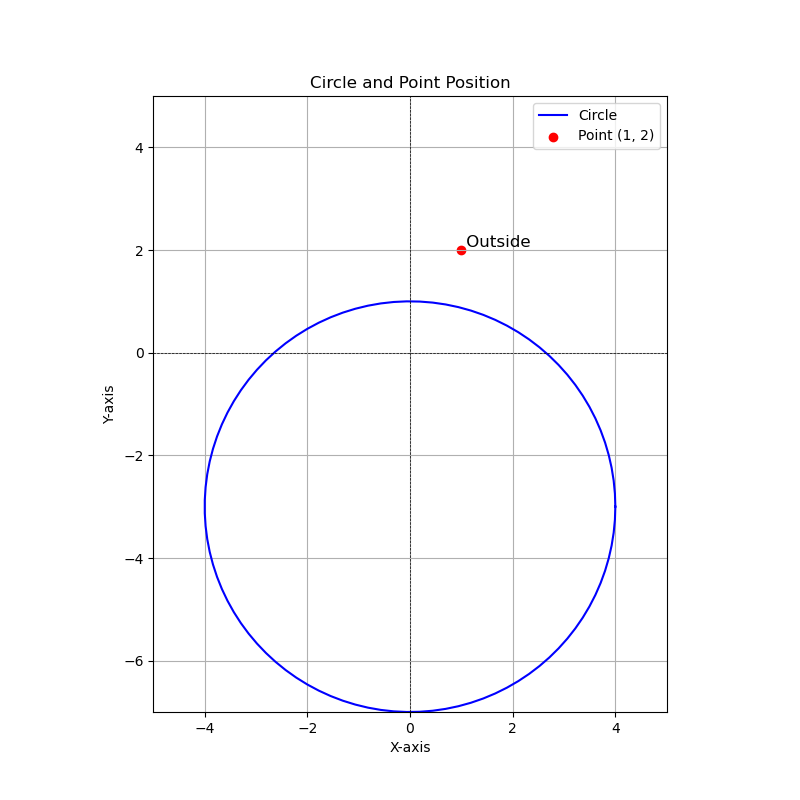
\includegraphics[width=0.7\linewidth]{figure/Figure_1.png}
	\caption{Circle}
\end{figure}

\end{document}
